\section{Introduction}
Music information can be very complex. Describing a classical masterpiece in all its form (the composition, the score, the various publications, a performance, a recording, the derivative works, etc.) is a complex activity. An even more challenging task consists in describing jazz and ethnic music for which the performance plays a central role, the music is generally not written and the authorship is not well defined. In the context of the DOREMUS research project\footnote{url{http://www.doremus.org}}, we develop tools and methods to manage music catalogues on the web using semantic web technologies. 

In this tutorial, we show strategies and tools for managing music knowledge. In the Section~\ref{sec:model}, we present the DOREMUS model for describing music, together with music specific controlled vocabularies. In the Section~\ref{sec:convert}, we present tools for converting music datasets, taking as example the ones coming from the rich musical archives of three leading cultural institutions in France -- the Biblioth\`eque Nationale de France (BnF), the Philharmonie de Paris (PP) and Radio France (RF) -- describing musical works, publications, performances and concerts. We demonstrate the expressiveness of the model showing  how complex music-specific queries can be answered. Finally, we describe strategies for data visualisation and recommendation in the Section~\ref{sec:explore}.

\section{A music data model}\label{sec:model}
Among the music ontologies, the most known example is the Music Ontology~\cite{raimond2007music} that provides a set of music-specific classes and properties for describing musical works, performances and tracks, together with fragments of them. Further needs in exploit the music knowledge coming from libraries led to the definition of a new ontology.

\subsection{The DOREMUS Ontology}
The DOREMUS model\footnote{\url{http://data.doremus.org/ontology/}} is an extension of FRBRoo, for describing cultural objects~\cite{doerr2008frbroo}, applied to the specific domain of music. This is a dynamic model, in which the abstract intention of the author (called Work) exists only through an Event (i.e. the composition event) that realises it in a distinct series of choices called Expression. This Work-Expression-Event triplet can also describe different parts of the life of a work, like the Performance, the Publication or the creation of a derivative Work, each one incorporating the expression from which it comes from.

On top of the FRBRoo original classes and properties, specific ones have been added in order to describe aspects of a work that are specifically related to music, such as the musical key, the genre, the tempo, the medium of performance (MoP), etc.~\cite{choffe2016doremus}.

Each triplet contains an information that, at the same time, can live autonomously and be linked to the other entities. Thinking about a classic work, we will have a triplet for the composition, one for any performance event, one for every manifestation (i.e. the score), etc., all connected in the graph. A jazz improvisation that consists in an extemporaneous creation of a new work, will have only the triplet for the Performance Work, Performance Expression and Performance Creation, in absence of the moment of composition and writing of the score that are almost mandatory for classical music and without the need to be attached to any other entity. It is considered a work \textit{per se}. All the Work entities of each triplet are then connected to a Complex Work, a class that has the objective of collecting together all the representations --- both the conceptual and sensory ones (manifestation) --- of the same creative idea.

The result is a model that, if on one side is quite complex and hard to adopt, on the other hand has a very detailed expressiveness. The graph depicted in\figref{fig:schema} shows a real example from our data: Beethoven's \textit{Sonata for piano and cello n.1}\footnote{\url{http://data.doremus.org/expression/614925f2-1da7-39c1-8fb7-4866b1d39fc7}}.

\begin{figure*}
 \centerline{
 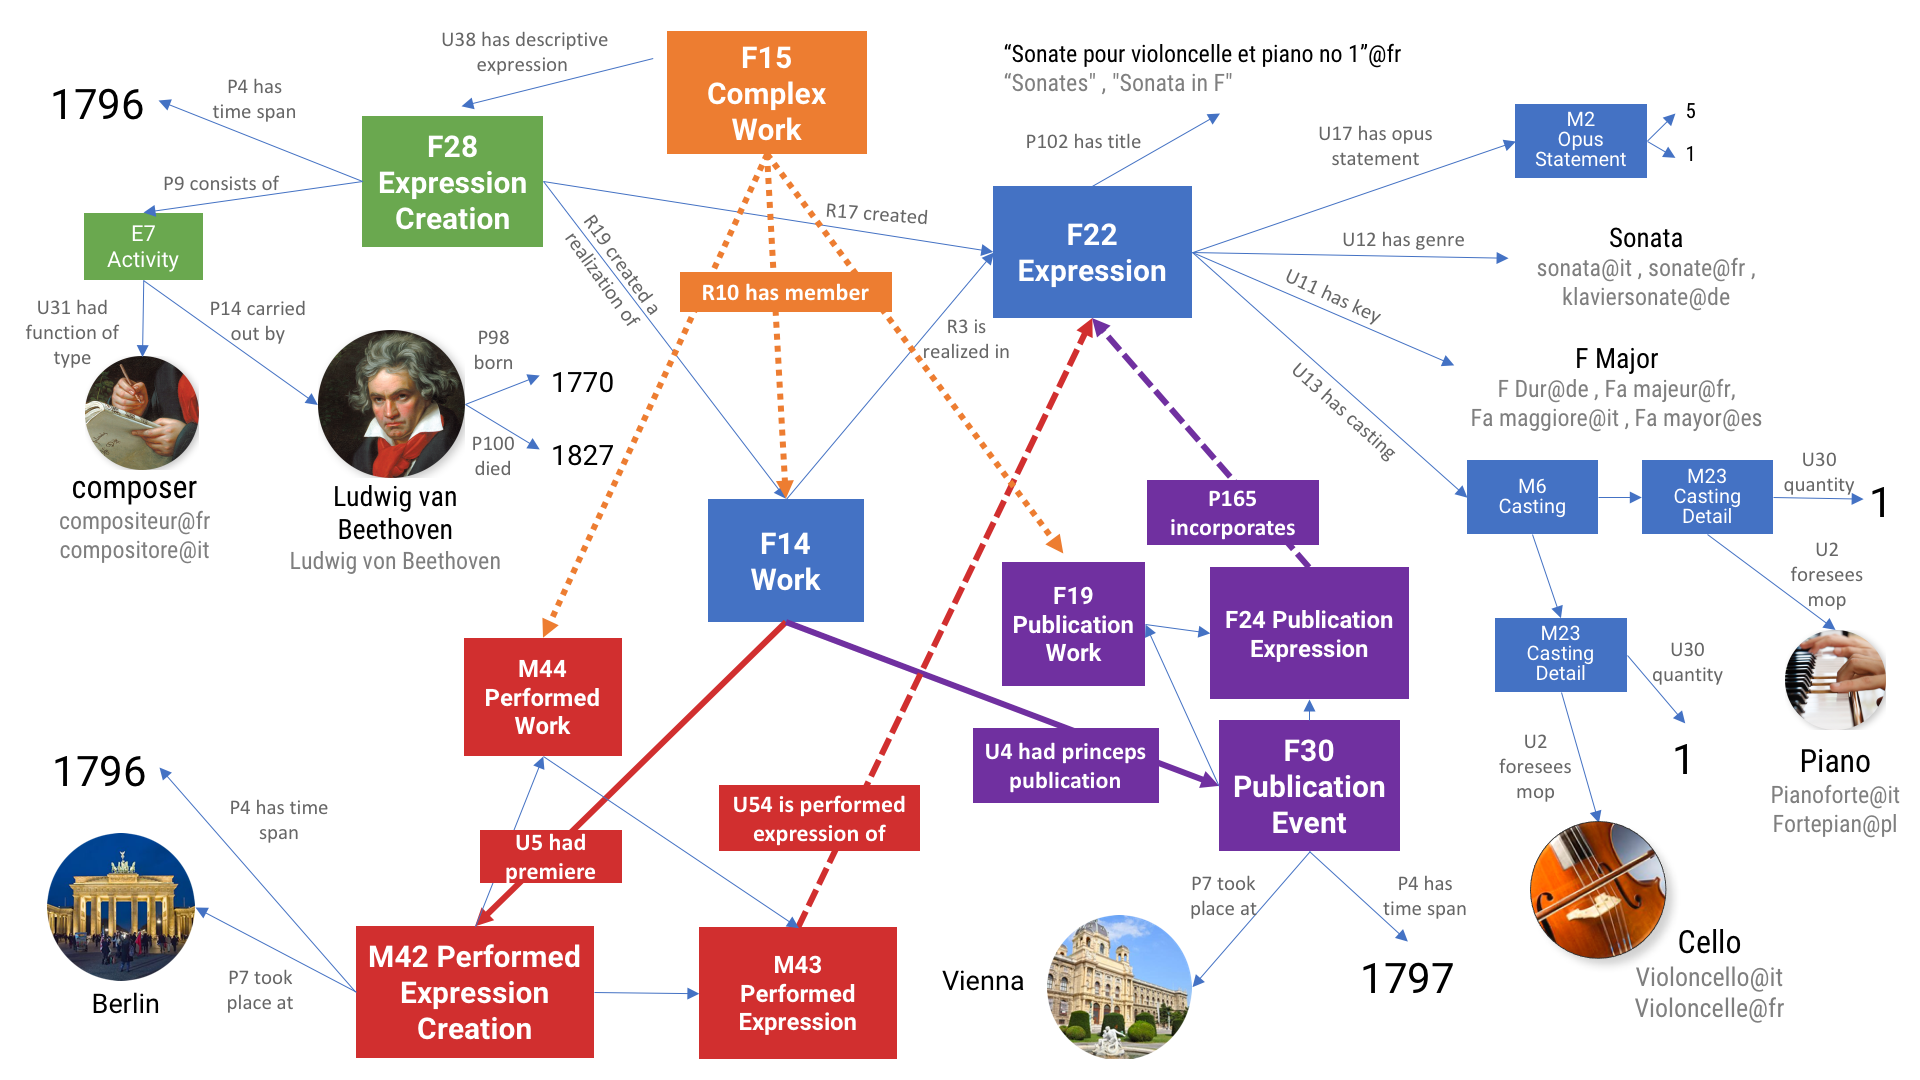
\includegraphics[width=\textwidth]{figs/schema_2.png}}
 \caption{Beethoven's \textit{Sonata for piano and cello n.1} represented as a graph using the DOREMUS ontology}
 \label{fig:schema}
\end{figure*}

\subsection{Music Controlled Vocabularies}
A large number of properties that are involved in the music description are supposed to contain values that are shared among different entities: different composition can have as genre ``sonata'', different performer can play a ``bassoon'', different authors can have as function ``composer'' or ``lyricist''. These labels can be expressed in multiple languages or in alternative forms (i.e. ``sax'' and ``saxophone'', or the French keys "Do majeur" and "Ut majeur"), making reconciliation hard. Our choice is to use controlled vocabularies for those common concepts. A controlled vocabulary is a thematic thesaurus of entities, each one being again identified with a URI. We are using SKOS~\cite{miles2007skos} as representation model, that allows to specify for each concept the preferred and the alternative labels in multiple language, to define a hierarchy between the concepts (so that the ``violin'' is a narrower concept with respect to ``string''), and to add comments and notes for describing the entity and help the annotation activity. Each concept becomes a common node in the musical graph that can connect a musical work to another, an author to a performer, etc.

Different kinds of vocabularies are required for describing music.
Some of them are already available on the web: this is the case of MIMO\footnote{\url{http://www.mimo-db.eu/}} for describing musical instruments, or RAMEAU\footnote{\url{http://rameau.bnf.fr/}} for musical genres, ethnic groups, etc. Some others are not published in a suitable format for the Web of Data, or the version published is not as complete as other formats that are available to libraries or in online sources: this happens with the vocabularies published by the International Association of Music Libraries (IAML), \footnote{\url{http://iflastandards.info/ns/unimarc/}} that have been published after the start of the project and for which we sometimes provide more details (labels, languages, etc.). Finally, there is also the case of vocabularies that do not exist at all and that we generate on the base of real data coming from the partners, enriched by an editorial process that involved also librarians. As a result, we collected, implemented and published 15 controlled vocabularies belonging to 6 different categories\footnote{\url{https://github.com/DOREMUS-ANR/knowledge-base/tree/master/vocabularies}}.

\section{Data Conversion}\label{sec:convert}
Both the French National Library (BnF) and Philharmonie of Paris make use of the MARC format for representing the music metadata. The flat structure of MARC, which consists in a succession of fields and subfields (\figref{fig:unimarc}), reflects the purpose of converting printed or handwritten records in a computer form. Although MARC is a standard, its adoption is restricted to the library world, making its serialization to other formats (usually XML) a need for an actual use. MARC fields are also not labeled explicitly, but encoded with numbers, with the consequence of having to use a manual for deciphering the content. The semantics of these fields and subfields is not trivial: a subfield can change its meaning depending on the field, under which it is found, and on the particular variant of MARC (UNIMARC and INTERMARC). A field or subfield can contain information about different entities, like the first performance and the first publication combined in the same field of the notes, without a clear separation. Often, the information is represented in the form of a free text~\cite{tennant2002marc}.

The benefits of moving from MARC to an RDF-based solution consist in the interoperability and the integration among libraries and with third party actors, with the possibility of realizing smart federated search~\cite{byrne2010strongest, alemu2012linked}. In order to achieve these goals, two tasks are necessary: data conversion and data linking.

\subsection{From MARC to RDF}
For the conversion task, we rely on \smallsc{marc2rdf}, \footnote{\url{https://github.com/DOREMUS-ANR/marc2rdf}} an open source prototype we developed for the automatic conversion of MARC bibliographic records to RDF using the DOREMUS ontology~\cite{lisena2016exploring}. The conversion process relies on explicit expert-defined transfer rules (or mappings) that indicate where in the MARC file to look for what kind of information, providing the corresponding property path in the model as well as useful examples that illustrate each transfer rule, as shown in~\figref{fig:mappings}. The role of these rules goes beyond being a simple documentation for the MARC records, embedding also information on some librarian practices in the formalisation of the content (format of dates, agreements on the syntax of textual fields, default values if the information is absent).

The converter is composed of different modules, that works in succession. First, a \textit{file} parser reads the MARC file and makes the content accessible by field and subfield number. We implemented a converting module for both the INTERMARC and UNIMARC variants. Then, it builds the RDF graph reading the fields and assigning their content to the DOREMUS property suggested in the transfer rules.

Then the \textit{free-text interpreter} extracts further information from the plain text fields, that includes editorial notes.This amounts to do a knowledge-aware parsing, since we search in the string exactly the information we want to instantiate from the model (i.e. the MoP from the casting notes, or the date and the publisher from the first publication note). The parsing is realized through empirically defined regular expression, that are going to be supported by Named Entity Recognition techniques as a future work. Finally, the \textit{string2vocabulary} component performs an automatic mapping of string literals to URIs coming from controlled vocabularies. All variants for a concept label are considered in order to deal with potential differences in naming terms. As additional feature, this component is able to recognise and correct some noise that is present in the source MARC file: this is the case of musical keys declared as genre, or fields for the opus number that contain actually a catalog number and vice-versa. These cases and other typos and mistakes have been identified thanks to the conversion process and the visualization of the converted data, supporting the source institution in they work of updating and correcting constantly their data.

\begin{figure}
 \centerline{\framebox{
  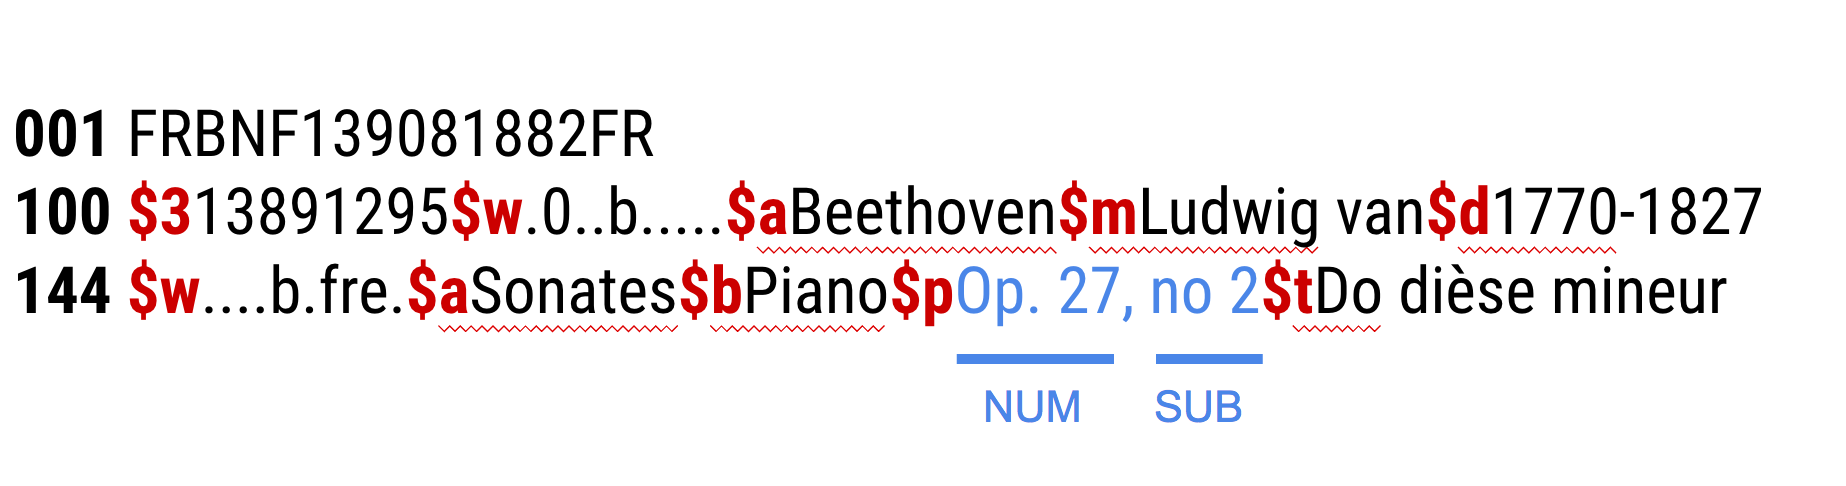
\includegraphics[width=6cm]{figs/MARC_example.png}}}
  \caption{An excerpt of a UNIMARC record.}
 \label{fig:unimarc}
 \smallskip
 \centerline{\framebox{
  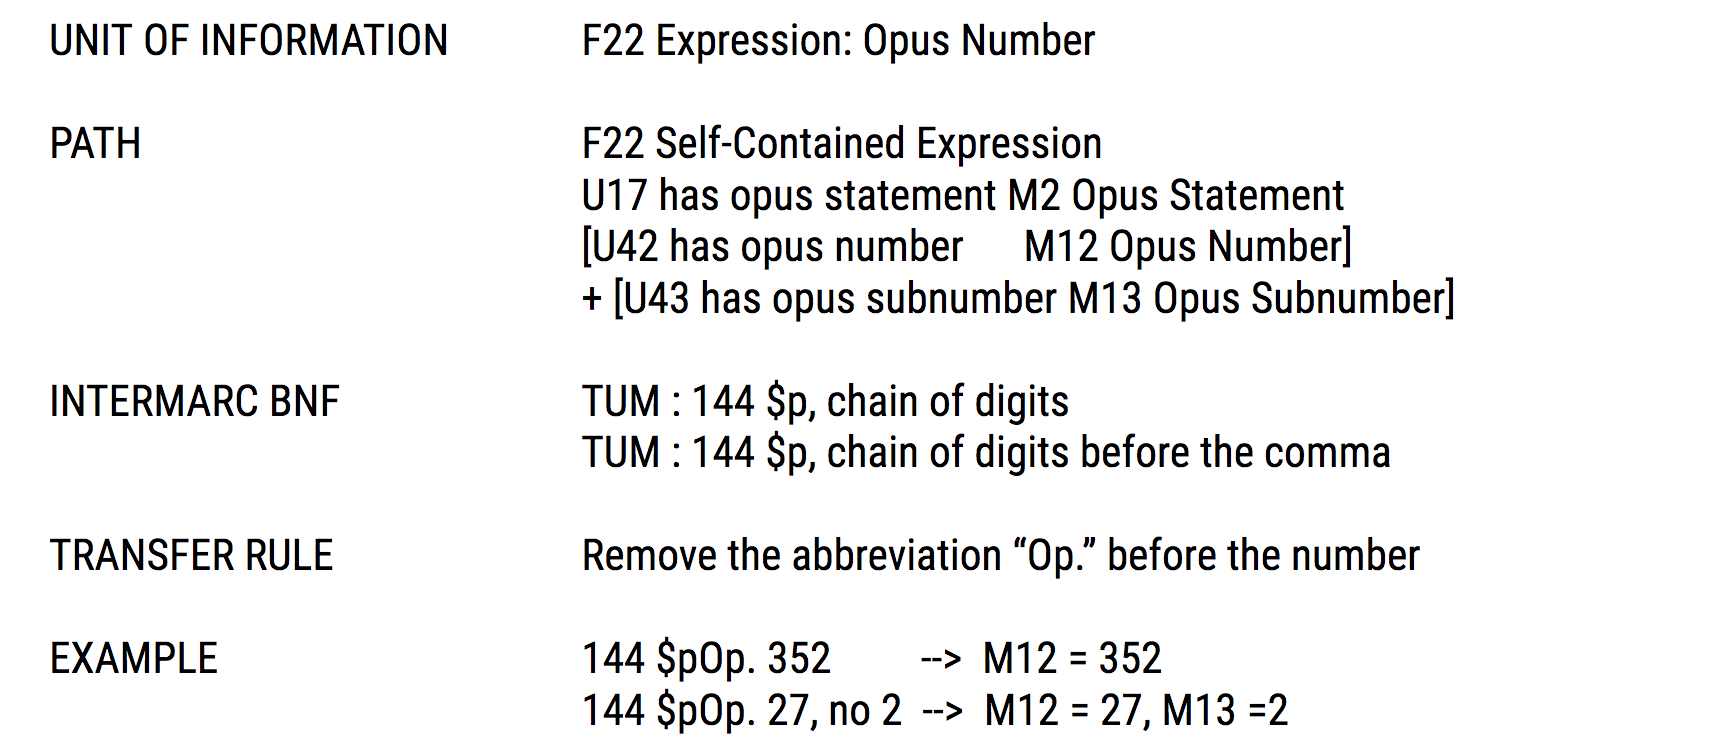
\includegraphics[width=\columnwidth]{figs/mapping_rule.png}}}
  \caption{Example of mapping rules describing the opus number and sub-number of a work}
 \label{fig:mappings}
\end{figure}

\subsection{Dealing With Heterogeneous Formats}
Apart from MARC, we are converting other source bases (in XML), that are too specific to be handled by a single converter. Therefore, we developed \textit{ad hoc} software that have a generic workflow: parse the input file and collect the required information, create the graph structure in RDF, run the \textit{string2vocabulary} module described previously. This procedure creates different graphs, one for each source. Those source databases are complementary but also contain overlaps (e.g. two databases that describe the same work or the same performance with complementary metadata). We have started to automatically interlink the datasets, so that the resulting knowledge graph provides a richer description of each work.

\subsection{Answering complex queries}
Before the beginning of the project, a list of questions have been collected from experts of the partner institutions\footnote{\url{https://github.com/DOREMUS-ANR/knowledge-base/tree/master/query-examples}}. These questions reflect real needs of the institutions and reveal problems that they face daily in the task of selecting information from the database (e.g. concert organisation or broadcast programming) or for supporting librarian and musicologist studies. They can be related to practical use cases (the search of all the scores that suit a particular formation), to musicologist topics (the music of a certain region in a particular historical period), to interesting stats (the works usually performed or published together), or to curious connections between works, performances or artists. Most of the questions are very specific and complex, so that it is very hard to find their answer by simply querying the search engines currently available on the web. We have grouped these questions in categories, according to the DOREMUS classes involved in the question.

% Among them, we can find questions that overflow the model, because they contain aspects that go beyond the music information and involve other kind of knowledge. An example is \textit{Retrieve a list of works of chamber music composed in the 19\textsuperscript{th} century by Scandinavian composers}: it requires knowledge of the birth place of the composer, and if this place is located in one of the Scandinavian countries. We can state that these are very interesting questions, because they are the ones that can fully exploit the advantages of linked data technologies. In fact, this kind of queries are quite far from having an answer in a traditional data storing system (e.g. database). The Web of Data gives the possibility of performing federated queries involving the Linked Open Data cloud (LOD), in particular datasets such as Geonames or DBpedia. For this reasons, the interconnection of the data is crucial. 

\tabref{tab:queries} provides an overview of how many queries we can currently write for each category. The implementation of recordings, scores, performance that is still work in progress -- along with the interconnection to the LOD repositories -- is one important reason for which some questions have not yet been translated into SPARQL and other ones have not results. 

\begin{table}
 \begin{center}
 \begin{tabular}{|l|c|}
  \hline
  Category & Query~/~Questions \\
  \hline
  A. Works & 23 / 29 \\
  \hline
  B. Artists & 1 / 3 \\
  \hline
  C. Performances & 6 / 9 \\
  \hline
  D. Recordings & 0 / 11 \\
  \hline
  E. Publications & 0 / 5 \\
  \hline
 \end{tabular}
\end{center}
 \caption{For each category of questions, we provide the ratio of the number of converted queries}
 \label{tab:queries}
\end{table}

\section{Exploration and Recommendation}\label{sec:explore}
We consider exploration and recommendation as two sides of the same medal. With the first one, we let the user browse the datasets, discover connections on his own, understand how we build the knowledge. Through recommendation, we remove this responsibility to the user with the purpose of presenting what he needs in a particular moment.

\subsection{Visualizing the Complexity}
We developed the first version of \textsc{Overture}, a web prototype of an exploratory search engine for DOREMUS data. The application makes requests directly to our SPARQL endpoint\footnote{\url{http://data.doremus.org/sparql}} and provides the information in a nice user interface.

At the top of the user interface, the navigation bar allows the user to navigate between the main concepts of the DOREMUS model: expression, performance, score, recording, artist. The challenge is in giving to the final user a complete vision on the data of each class and letting him/her understand how they are connected to each other. We keep as example Beethoven's \textit{Sonata for piano and cello n.1} \footnote{\url{http://overture.doremus.org/expression/614925f2-1da7-39c1-8fb7-4866b1d39fc7}}. Aside from the different versions of the title, the composer and a textual description, the page provides details on the information we have about the work, like the musical key, the genres, the intended MoP, the opus number. When these values come from a controlled vocabulary, a link is presented in order to search for expressions that share the same value (for example, the same genre or the same musical key). A timeline shows the most important events related to the work (the composition, the premiere, the first publication). Other performances and publications can be represented below. 
The background is a portrait of the composer that comes from DBpedia. It is retrieved thanks to the presence in the DOREMUS database of \texttt{owl:sameAs} links. These links comes in part from the International Standard Name Identifier (ISNI) service\footnote{The ISNI database contains authority information about people involved in creative processes (i.e. artists). It is managed by the ISNI Quality Team, which the BnF is a member of, and artists record in the BnF database contains generally an ISNI reference.}, in part thanks to an interlinking realised by matching the artist name, birth and death date in the different datasets.

\subsection{Music Recommendation Using Graph Embeddings}
What should we suggest to a user listening Beethoven? Similar musicians should share with the German composer some features: the period, similar properties on the compositions (genre, key, casting) or similar instrument played (the piano itself, or also the harpsichord that is in the same family). But how to define a similarity measure that take into acount these concepts? We propose a solution based on graph embeddings generated at different levels:
\begin{enumerate}
  \item For simple features (e.g. genre, key, instrument), we compute for each term an embedding applying \textit{node2vec}~\cite{node2vec-kdd2016} on two sub-graphs: the one of the controlled vocabularies and the one corresponding to the usage of their values in the DOREMUS dataset;
  \item For complex features (e.g. artist), we generate the embeddings by the combination of its corresponding feature embedding. In the case of artists, we will generate a vector composed of the period (mapped in $[0,1]$) and the averages of the vector of the genre, key and casting (instrument) of his composition, together with the one of the played instrument, after having reduced their dimensionality;
  \item Finally, for the work, we combine again simple and complex feature embedding, following the same rules.
\end{enumerate}

Using graph embeddings reduces the similarity problem as the reverse of an euclidean distance. if some properties are missing, we apply a penalisation computed as percentage of missing feature in the target vector with respect to the seed one~\cite{lisena2017combining}.

The biggest advantage of this method is that the embeddings computation is required only for the simple features: each embedding is re-used in different combination. Because different weights can be assigned to each property in order to tune up the recommendation, we plan to experiment with neural networks in order to discover the best weighting strategy.

\begin{acks}
This work has been partially supported by the French National Research Agency (ANR) within the DOREMUS Project, under grant number ANR-14-CE24-0020.
\end{acks}
